\documentclass[11pt]{article}

\usepackage{amsmath,amssymb,amsfonts}
\usepackage{graphicx}
\usepackage{pgfplots}
\usepackage{multicol}
\usepackage{enumitem}
\usepgfplotslibrary{fillbetween}
\pgfplotsset{compat=1.16,width=10cm}


\setlength{\topmargin}{-.5in} \setlength{\textheight}{9.25in}
\setlength{\oddsidemargin}{0in} \setlength{\textwidth}{6.8in}


\begin{document}

\Large

\noindent{\bf Name: \hfill Date: \hfill Quiz 3 \hfill AP Calculus - Hargus}

\medskip\hrule
\vspace{10pt}

\begin{enumerate}

\item (10 points) Label each section on the following graph of $f(x)$ with the sign combination of $f'(x)$ and $f''(x)$, in that order.  (For example,  between $A$ and $B$ you would write $++$ because $f'(x) > 0$ and $f''(x) > 0$)

\begin{center}
\tikzset{every picture/.style={line width=0.75pt}} %set default line width to 0.75pt        

\begin{tikzpicture}[x=0.75pt,y=0.75pt,yscale=-1,xscale=1]
%uncomment if require: \path (0,300); %set diagram left start at 0, and has height of 300

%Curve Lines [id:da4288999458582473] 
\draw    (98,142) .. controls (106.91,154) and (142.54,165) .. (204.89,118) .. controls (267.24,71) and (335.53,114) .. (351.86,137) ;
%Curve Lines [id:da3575185057246374] 
\draw    (351.86,137) .. controls (368.06,107.71) and (402.33,76) .. (429.05,94) .. controls (455.77,112) and (476.56,183) .. (506.25,153) ;
%Shape: Ellipse [id:dp167375923089641] 
\draw  [fill={rgb, 255:red, 74; green, 144; blue, 226 }  ,fill opacity=1 ] (123.24,152.5) .. controls (123.24,150.57) and (124.75,149) .. (126.62,149) .. controls (128.49,149) and (130,150.57) .. (130,152.5) .. controls (130,154.43) and (128.49,156) .. (126.62,156) .. controls (124.75,156) and (123.24,154.43) .. (123.24,152.5) -- cycle ;
%Straight Lines [id:da8741969117493095] 
\draw    (102.45,197) -- (522.58,197) -- (527,197) ;
\draw [shift={(530,197)}, rotate = 180] [fill={rgb, 255:red, 0; green, 0; blue, 0 }  ][line width=0.08]  [draw opacity=0] (8.93,-4.29) -- (0,0) -- (8.93,4.29) -- cycle    ;
%Straight Lines [id:da1548512712530017] 
\draw    (109.88,219) -- (109.88,55) ;
\draw [shift={(109.88,52)}, rotate = 450] [fill={rgb, 255:red, 0; green, 0; blue, 0 }  ][line width=0.08]  [draw opacity=0] (8.93,-4.29) -- (0,0) -- (8.93,4.29) -- cycle    ;
%Shape: Ellipse [id:dp785294152446717] 
\draw  [fill={rgb, 255:red, 74; green, 144; blue, 226 }  ,fill opacity=1 ] (190.24,125.5) .. controls (190.24,123.57) and (191.75,122) .. (193.62,122) .. controls (195.49,122) and (197,123.57) .. (197,125.5) .. controls (197,127.43) and (195.49,129) .. (193.62,129) .. controls (191.75,129) and (190.24,127.43) .. (190.24,125.5) -- cycle ;
%Shape: Ellipse [id:dp5547564941014383] 
\draw  [fill={rgb, 255:red, 74; green, 144; blue, 226 }  ,fill opacity=1 ] (263.24,97.5) .. controls (263.24,95.57) and (264.75,94) .. (266.62,94) .. controls (268.49,94) and (270,95.57) .. (270,97.5) .. controls (270,99.43) and (268.49,101) .. (266.62,101) .. controls (264.75,101) and (263.24,99.43) .. (263.24,97.5) -- cycle ;
%Shape: Ellipse [id:dp7252140248830908] 
\draw  [fill={rgb, 255:red, 74; green, 144; blue, 226 }  ,fill opacity=1 ] (348.86,137) .. controls (348.86,135.07) and (350.37,133.5) .. (352.24,133.5) .. controls (354.1,133.5) and (355.62,135.07) .. (355.62,137) .. controls (355.62,138.93) and (354.1,140.5) .. (352.24,140.5) .. controls (350.37,140.5) and (348.86,138.93) .. (348.86,137) -- cycle ;
%Shape: Ellipse [id:dp5213980426397898] 
\draw  [fill={rgb, 255:red, 74; green, 144; blue, 226 }  ,fill opacity=1 ] (408.24,89.5) .. controls (408.24,87.57) and (409.75,86) .. (411.62,86) .. controls (413.49,86) and (415,87.57) .. (415,89.5) .. controls (415,91.43) and (413.49,93) .. (411.62,93) .. controls (409.75,93) and (408.24,91.43) .. (408.24,89.5) -- cycle ;
%Shape: Ellipse [id:dp37869629849705655] 
\draw  [fill={rgb, 255:red, 74; green, 144; blue, 226 }  ,fill opacity=1 ] (451.24,125.5) .. controls (451.24,123.57) and (452.75,122) .. (454.62,122) .. controls (456.49,122) and (458,123.57) .. (458,125.5) .. controls (458,127.43) and (456.49,129) .. (454.62,129) .. controls (452.75,129) and (451.24,127.43) .. (451.24,125.5) -- cycle ;
%Shape: Ellipse [id:dp8737945641450182] 
\draw  [fill={rgb, 255:red, 74; green, 144; blue, 226 }  ,fill opacity=1 ] (487.24,160.5) .. controls (487.24,158.57) and (488.75,157) .. (490.62,157) .. controls (492.49,157) and (494,158.57) .. (494,160.5) .. controls (494,162.43) and (492.49,164) .. (490.62,164) .. controls (488.75,164) and (487.24,162.43) .. (487.24,160.5) -- cycle ;
%Straight Lines [id:da9757461842357297] 
\draw  [dash pattern={on 4.5pt off 4.5pt}]  (126.62,152.5) -- (126,197) ;
%Straight Lines [id:da4907242482500207] 
\draw  [dash pattern={on 4.5pt off 4.5pt}]  (193.62,125.5) -- (194,197) ;
%Straight Lines [id:da4363425352088973] 
\draw  [dash pattern={on 4.5pt off 4.5pt}]  (266.62,97.5) -- (267,197) ;
%Straight Lines [id:da4949518088803153] 
\draw  [dash pattern={on 4.5pt off 4.5pt}]  (352.24,137) -- (352.62,196.5) ;
%Straight Lines [id:da1146912923263097] 
\draw  [dash pattern={on 4.5pt off 4.5pt}]  (411.62,89.5) -- (412,197) ;
%Straight Lines [id:da4268299707103482] 
\draw  [dash pattern={on 4.5pt off 4.5pt}]  (454.62,125.5) -- (455,197) ;
%Straight Lines [id:da014192954392583057] 
\draw  [dash pattern={on 4.5pt off 4.5pt}]  (490.62,160.5) -- (491,197) ;
%Straight Lines [id:da7163959962951796] 
\draw    (146,245) -- (173,245) ;
%Straight Lines [id:da7006190252587259] 
\draw    (213,245) -- (240,245) ;
%Straight Lines [id:da03981546449838991] 
\draw    (297,245) -- (324,245) ;
%Straight Lines [id:da38615921219722604] 
\draw    (370,245) -- (397,245) ;
%Straight Lines [id:da8425255855958811] 
\draw    (419,245) -- (446,245) ;
%Straight Lines [id:da29351552433243655] 
\draw    (462,245) -- (489,245) ;

% Text Node
\draw (117.39,198.4) node [anchor=north west][inner sep=0.75pt]    {$A$};
% Text Node
\draw (187.98,198.4) node [anchor=north west][inner sep=0.75pt]    {$B$};
% Text Node
\draw (259.72,198.4) node [anchor=north west][inner sep=0.75pt]    {$C$};
% Text Node
\draw (344.58,198.4) node [anchor=north west][inner sep=0.75pt]    {$D$};
% Text Node
\draw (404.72,198.4) node [anchor=north west][inner sep=0.75pt]    {$E$};
% Text Node
\draw (447.77,198.4) node [anchor=north west][inner sep=0.75pt]    {$F$};
% Text Node
\draw (482.64,198.4) node [anchor=north west][inner sep=0.75pt]    {$H$};
% Text Node
\draw (143,223) node [anchor=north west][inner sep=0.75pt]    {$++$};


\end{tikzpicture}
\end{center}

\item (10 points) Write an expression for the gray area below between $y=\frac{1}{x}$ and $y=\frac{1}{2}$ from $x=1$ to $x=3$.  An expression using integral(s) is okay here, you \textbf{do not} need to calculate the answer.

\begin{center}
\begin{tikzpicture}[declare function={a=1;b=3;f(\x)=1/\x;g(\x)=0.5;}]
 \begin{axis}[axis lines=middle,axis on top,xlabel=$x$,ylabel=$y$,
 xmin=-0.5,xmax=5,ymin=-0.5,ymax=2,ytick=\empty,
 xtick={a,2,b},xticklabels={$1$,$2$,$3$}, 
 every axis x label/.style={at={(current axis.right of origin)},anchor=north west},
 every axis y label/.style={at={(current axis.above origin)},anchor=north east}]
  \addplot[name path=A,blue,thick,domain=0.2:5,smooth,] {f(x)}
  node [pos=0.4, right] {$y=\frac{1}{x}$};
  \addplot[name path=B,purple,thick,domain=0.2:5,smooth] {g(x)}
  node [pos=0.8, above] {$y=\frac{1}{2}$};
  \path[name path=C] (\pgfkeysvalueof{/pgfplots/xmin},0) -- (\pgfkeysvalueof{/pgfplots/xmax},0);
    \addplot [gray] fill between [
        of=A and B,soft clip={domain=1:b},
    ];
 \end{axis}
\end{tikzpicture}
\end{center}

\vspace{50pt}
\begin{center}
Area $=$ \rule{10cm}{0.4pt}
\end{center}

\newpage

\item (10 points) Given that the area $A_1 = 5$ and $\int_{a}^{b}f(x) dx = 11$, what is $A_2$ in the graph below?

\begin{center}
\begin{tikzpicture}[declare function={a=0.5;b=3;f(\x)=1/\x;}]
 \begin{axis}[axis lines=middle,axis on top,xlabel=$x$,ylabel=$y$,
 xmin=-0.5,xmax=5,ymin=-0.5,ymax=2,ytick=\empty,
 xtick={a,1,b},xticklabels={$a$,$4$,$b$}, 
 every axis x label/.style={at={(current axis.right of origin)},anchor=north west},
 every axis y label/.style={at={(current axis.above origin)},anchor=north east}]
 \addplot[name path=A,blue,thick,domain=0.2:5,smooth,] {f(x)}
  node [pos=0.4, right] {$f(x)$};
  \addplot[name path=A,blue,thick,domain=0.2:5,smooth] {f(x)};
  \path[name path=B] (\pgfkeysvalueof{/pgfplots/xmin},0) -- (\pgfkeysvalueof{/pgfplots/xmax},0);
  \addplot [gray!30] fill between [
        of=A and B,soft clip={domain=a:1},
    ];
    \addplot [gray] fill between [
        of=A and B,soft clip={domain=1:b},
    ];
    \path ({(1+a)/2},{f((1+a)/2)/2}) node{$A_1$}
    ({(1+b)/2},{f((1+b)/2)/2}) node{$A_2$};
 \end{axis}
\end{tikzpicture}
\end{center}

\vspace{20pt}
\begin{flushright}
$A_2 = $ \rule{2cm}{0.4pt}
\end{flushright}


\item (10 points) Solve the integral.
\begin{enumerate}[itemsep=25pt]
    \item $\int \cos(x)dx = $ \\
    \item $\int (4x^2 - 2e^x)dx  =$ \\
\end{enumerate}

\vspace{10 mm}

\item (10 points) Suppose that $f'(3)=0$.  If $f''(3) < 0$, what does the graph of $f(x)$ have at $x=3$? (circle one answer)
\begin{enumerate}
    \item Maximum
    \item Minimum
    \item Point of inflection
\end{enumerate}


\newpage

\item (20 points) Find the critical points for the function $f(x) = x^3 - 4x^2 +4x+1$. Then, find the transition points and draw a sign chart for $f'(x)$ and $f''(x)$ showing the intervals where each function is positive or negative. Then, use this information to sketch the graph $f(x)$ below (label any minimums, maximums, and points of inflection).
\\

\vspace{60 mm}

\vspace{10pt}
\begin{center}
\begin{tikzpicture}
\begin{axis}[ xlabel={$x$}, ylabel={$y$}
  ,axis lines=middle
  ,samples=500, grid, thick
  ,domain=-10:10
  ,axis equal
  ,legend pos=outer north east
  ,xmin=-1, xmax=4,
  ,ymin=-1, ymax=4
  ]
\addplot+[no marks] {-10};
\end{axis}
\end{tikzpicture}
\end{center}


\end{enumerate}

\end{document} 